\documentclass[11pt,a4paper,twoside]{tesis}
% SI NO PENSAS IMPRIMIRLO EN FORMATO LIBRO PODES USAR
%\documentclass[11pt,a4paper]{tesis}

\usepackage{graphicx}
\graphicspath{ {images/} }
\usepackage[utf8]{inputenc}
\usepackage[spanish]{babel}
\usepackage[left=3cm,right=3cm,bottom=3.5cm,top=3.5cm]{geometry}
\usepackage{amsthm}
\usepackage[T1]{fontenc}
\newtheorem{exmp}{Ejemplo}



\begin{document}

%%%% CARATULA

\def\autor{Pablo Víctor Fromer}
\def\tituloTesis{Datalog +/-, \vspace{.2cm} \\ una interfaz tolerante a la inconsistencia }
\def\runtitulo{Datalog +/-, una interfaz tolerante a la inconsistencia}
\def\runtitle{Datalog +/-, una interfaz tolerante a la inconsistencia}
\def\director{María Vanina Martinez}
\def\codirector{Ricardo Oscar Rodriguez}
\def\lugar{Buenos Aires, 2019}
\newcommand{\HRule}{\rule{\linewidth}{0.2mm}}
%
\thispagestyle{empty}

\begin{center}\leavevmode

\vspace{-2cm}

\begin{tabular}{l}

\includegraphics[width=2.6cm]{logofcen.pdf}
\end{tabular}


{\large \sc Universidad de Buenos Aires

Facultad de Ciencias Exactas y Naturales

Departamento de Computaci\'on}

\vspace{6.0cm}

%\vspace{3.0cm}
%{
%\Large \color{red}
%\begin{tabular}{|p{2cm}cp{2cm}|}
%\hline
%& Pre-Final Version: \today &\\
%\hline
%\end{tabular}
%}
%\vspace{2.5cm}

\begin{huge}
\textbf{\tituloTesis}
\end{huge}

\vspace{2cm}

{\large Tesis de Licenciatura en Ciencias de la Computaci\'on}

\vspace{2cm}

{\Large \autor}

\end{center}

\vfill

{\large

{Director: \director}

\vspace{.2cm}

{Codirector: \codirector}

\vspace{.2cm}

\lugar
}

\newpage\thispagestyle{empty}


%%%% ABSTRACTS, AGRADECIMIENTOS Y DEDICATORIA
%\frontmatter
%\pagestyle{empty}
%%\begin{center}
%\large \bf \runtitulo
%\end{center}
%\vspace{1cm}
\chapter*{\runtitulo}

\noindent La princesa Leia, líder del movimiento rebelde que desea reinstaurar la República en la galaxia en los tiempos ominosos del Imperio, es capturada por las malévolas Fuerzas Imperiales, capitaneadas por el implacable Darth Vader. El intrépido Luke Skywalker, ayudado por Han Solo, capitán de la nave espacial ``El Halcón Milenario'', y los androides, R2D2 y C3PO, serán los encargados de luchar contra el enemigo y rescatar a la princesa para volver a instaurar la justicia en el seno de la Galaxia (aprox. 200 palabras).

\bigskip

\noindent\textbf{Palabras claves:} Guerra, Rebelión, Wookie, Jedi, Fuerza, Imperio (no menos de 5).

%\cleardoublepage
%%\begin{center}
%\large \bf \runtitle
%\end{center}
%\vspace{1cm}
\chapter*{\runtitle}

\noindent In a galaxy far, far away, a psychopathic emperor and his most trusted servant -- a former Jedi Knight known as Darth Vader -- are ruling a universe with fear. They have built a horrifying weapon known as the Death Star, a giant battle station capable of annihilating a world in less than a second. When the Death Star's master plans are captured by the fledgling Rebel Alliance, Vader starts a pursuit of the ship carrying them. A young dissident Senator, Leia Organa, is aboard the ship \& puts the plans into a maintenance robot named R2-D2. Although she is captured, the Death Star plans cannot be found, as R2 \& his companion, a tall robot named C-3PO, have escaped to the desert world of Tatooine below. Through a series of mishaps, the robots end up in the hands of a farm boy named Luke Skywalker, who lives with his Uncle Owen \& Aunt Beru. Owen \& Beru are viciously murdered by the Empire's stormtroopers who are trying to recover the plans, and Luke \& the robots meet with former Jedi Knight Obi-Wan Kenobi to try to return the plans to Leia Organa's home, Alderaan. After contracting a pilot named Han Solo \& his Wookiee companion Chewbacca, they escape an Imperial blockade. But when they reach Alderaan's coordinates, they find it destroyed - by the Death Star. They soon find themselves caught in a tractor beam \& pulled into the Death Star. Although they rescue Leia Organa from the Death Star after a series of narrow escapes, Kenobi becomes one with the Force after being killed by his former pupil - Darth Vader. They reach the Alliance's base on Yavin's fourth moon, but the Imperials are in hot pursuit with the Death Star, and plan to annihilate the Rebel base. The Rebels must quickly find a way to eliminate the Death Star before it destroys them as it did Alderaan (aprox. 200 palabras).

\bigskip

\noindent\textbf{Keywords:} War, Rebellion, Wookie, Jedi, The Force, Empire (no menos de 5). % OPCIONAL: comentar si no se quiere

%\cleardoublepage
%\chapter*{Agradecimientos}

\noindent Lorem ipsum dolor sit amet, consectetur adipiscing elit. Fusce sapien ipsum, aliquet eget convallis at, adipiscing non odio. Donec porttitor tincidunt cursus. In tellus dui, varius sed scelerisque faucibus, sagittis non magna. Vestibulum ante ipsum primis in faucibus orci luctus et ultrices posuere cubilia Curae; Mauris et luctus justo. Class aptent taciti sociosqu ad litora torquent per conubia nostra, per inceptos himenaeos. Mauris sit amet purus massa, sed sodales justo. Mauris id mi sed orci porttitor dictum. Donec vitae mi non leo consectetur tempus vel et sapien. Curabitur enim quam, sollicitudin id iaculis id, congue euismod diam. Sed in eros nec urna lacinia porttitor ut vitae nulla. Ut mattis, erat et laoreet feugiat, lacus urna hendrerit nisi, at tincidunt dui justo at felis. Class aptent taciti sociosqu ad litora torquent per conubia nostra, per inceptos himenaeos. Ut iaculis euismod magna et consequat. Mauris eu augue in ipsum elementum dictum. Sed accumsan, velit vel vehicula dignissim, nibh tellus consequat metus, vel fringilla neque dolor in dolor. Aliquam ac justo ut lectus iaculis pharetra vitae sed turpis. Aliquam pulvinar lorem vel ipsum auctor et hendrerit nisl molestie. Donec id felis nec ante placerat vehicula. Sed lacus risus, aliquet vel facilisis eu, placerat vitae augue.
 % OPCIONAL: comentar si no se quiere

%\cleardoublepage
%\hfill \textit{A mi persona favorita.}
  % OPCIONAL: comentar si no se quiere

\cleardoublepage
\tableofcontents

\mainmatter
\pagestyle{headings}

%%%% ACA VA EL CONTENIDO DE LA TESIS

\chapter{Introducción}
\section{Motivación Opcion 1}

Los lenguajes ontológicos, los sistemas basados en reglas y sus integraciones han jugado un rol central en el desarrollo de la Web Semántica…  Antes del surgimiento de Datalog +/- no existía literatura que explique cómo generalizar reglas y dependencias de bases de datos de manera que puedan expresar axiomas ontológicos. De esta manera no estaba cubierto el interés en la comunidad de la Web Semántica por conseguir formalismos altamente escalables que pudieran hacer que la red se beneficie de las tecnologías y las optimizaciones ya implementadas en los motores de bases de datos.

Datalog +/- es una serie de variantes del lenguaje Datalog que son particularmente adecuadas para responder consultas sobre ontologías de manera eficiente. Estas variantes extienden Datalog con la posibilidad de cuantificar existencialmente a las variables en las implicaciones de las reglas y otra serie de ventajas, mientras que al mismo tiempo restringen el lenguaje de manera sintáctica con el objetivo de asegurar tratabilidad.

Por otro lado, tanto en el campo de las bases de datos como en el de la Web Semántica es ampliamente reconocido que la inconsistencia es un problema que no puede ser ignorado. Al momento de integrar información proveniente de diversas fuentes, ya sea para popular una ontología o para responder una consulta, las restricciones de integridad son muy propensas a ser violadas en la práctica. En este trabajo proponemos una implementación de la semántica IAR, la cual describe un método para tratar ....

El objetivo de esta tesis es presentar una herramienta... una herramienta que tiene el propósito de acercar a la comunidad una implementación de Datalog+/-, con el objetivo de poder acceder a este lenguaje de manera fácil, a través de Internet...

\section{Datalog +/-}

En esta sección vamos a recordar los elementos principales del lenguaje Datalog (citar aca JWS).
Con respecto a los ingredientes elementales, se asumen constantes, nulos y variables de la siuguiente manera; estos son los arguentos de las fórmulas atómicas en las bases de datos, consultas y dependencias.
Se asume (i) un universo infinito de constantes  $\Delta$ (las cuáles forman el dominio de la base de  datos), (ii) un conjunto infinito de nulos etiquetados $\Delta_{N}$ (representando valores desconocidos), y (iii) un conjunto infinito de variables X (que se utilizan en las consultas y en las dependencias). Cada constante representa un valor diferente, mientras que nulos distintos podrían representar el mismo valor. 
Se asume un orden lexicográfico en  $\Delta \cup \Delta_{N}$, donde los símbolos de $\Delta_{N}$ siguen a los de $\Delta$. Se denota por $X$ a una sequencia de variables $X_{1}$, ..., $X_{K}$ con $k > 0$.

Se definen las fórmulas atómicas, que ocurren en bases de datos, consultas, y dependencias, y que se construyen en base a los nombres de las relaciones y los términos. Se asume un \textit{esquema relacional $R$}, el cual constituye un conjunto finito de \textit{nombres de relación}, o \textit{símbolos de predicado}. La posición \textit{P[i]} identifica al \textit{i}-esimo argumento de un predicado \textit{P}. Un \textit{término t} es una constante, un nulo o variable. Una \textit{fórmula atómica} (o \textit{átomo}) a tiene la forma \textit{P}($t_{1}$,...,$t_{n}$), donde \textit{P} es un predicado $n$-ario, y $t_{1}$,...,$t_{n}$ son términos. Se denotan por \textit{pred}(a) y \textit{dom}(a) su predicado y al conjunto de sus argumentos, respectivamente. Esta notación se extiende de manera natural para conjuntos y conjunciones de átomos. 

Podemos definir ahora la noción de base de datos relativa a un esquema relacional, junto con la sintaxis y la semántica de las consultas conjuntivas y las consultas conjuntivas booleanas a una base de datos. Una \textit{instancia de base de datos} $D$ para un esquema relacional $R$ es un conjunto de átomos (posiblemente infinito) con predicados de R y argumentos de $\Delta$. Una consulta conjuntiva sobre $R$ tiene la forma $Q(\textbf{X}) = \exists\textbf{Y}\Phi(\textbf{X},\textbf{Y})$, donde $\Phi(\textbf{X},\textbf{Y})$ es una conjunción de átomos con las variables \textbf{X} y \textbf{Y}, y eventualmente constantes, pero sin nulos. Una consulta conjuntiva \textit{Booleana} sobre $R$ es una consulta conjuntiva de la forma $Q() = \exists\textbf{Y}\Phi(\textbf{X},\textbf{Y})$, donde todas las variables están cuantificadas existencialmente. El conjunto de todas las respuestas a una consulta conjuntiva $Q(\textbf{X}) = \exists\textbf{Y}\Phi(\textbf{X},\textbf{Y})$ sobre una base de datos es el conjunto de todas las tuplas \textbf{t} sobre $\Delta$ para las cuales existe un homomorfismo $\mu: \textbf{X} \cup \textbf{X} \rightarrow \Delta \cup \Delta_{N}$ tales que $\mu(\Phi(\textbf{X},\textbf{Y})) \subseteq D$ y $\mu(\textbf{X}) = D$

\begin{exmp}\label{ejemplo_base_d}
Consideremos una base de datos de películas, que guarda información acerca de actores, directores y películas. El esquema relacional $R$ consite en los predicado unarios \textit{pelicula}, \textit{actor}, \textit{director},  y en los predicados binarios \textit{actuaEn}, \textit{dirigidaPor} y \textit{trabajaronJuntos}.  Una base de datos $D$ para el esquema  $R$ puede estar dada por: 
    \begin{equation}
        $$D = \{\textit{pelicula(Volver al Futuro),  pelicula(Esperando la carroza), actuaEn(Esperando la Carroza, Antonio Gasalla), actuaEn(Esperando la Carroza, China Zorrilla),
        actor(Antonio Gasalla), dirigidaPor(Esperando la Carroza, Alejandro Doria)}\}$$
    \end{equation}

Una posible consulta conjuntiva para esta base de datos podría ser Q(X) = pelicula(X) $\land$ actuaEn(X, Y), que pregunta por todas las películas en las que alguien haya actuado, cuya respuesta es el conjunto de una sola tupla $\{(Esperando la Carroza)\}$;  mientras que un ejemplo de consulta conjuntiva booleana es Q() =  actor(X) $\land$ actuaEn(Volver al Futuro, X), la cual pregunta si hay algún actor que haya actuado en Volver al Futuro, cuya respuesta en No.

\end{exmp}



\iffalse
$$D = \{\textit{pelicula(Esperando la carroza), pelicula(Volver al Futuro), pelicula(Thelma y Louise), actuaEn(Esperando la Carroza, Antonio Gasalla), actuaEn(Esperando la Carroza, China Zorrilla), actuaEn(Volver al futuro, Michael J. Fox), actuaEn(Thelma y Louise, Susan Sarandon), actuaEn(Thelma y Louise, Brad Pitt), dirigidaPor(Volver al Futuro, Robert Zemeckis)}\}$$
\fi



\subsection{Dependencias generadoras de tuplas (TGDs)}
Las dependencias generadoras de tuplas (TGDs) son restricciones sobre una base de datos en la forma general de las reglas de Datalog.....
Dado un esquema relacional $R$, una TGD $\sigma$ es una fórmula de primer orden de la forma $\forall X \forall Y \Phi (X, Y) \rightarrow \exists Z \Psi (X, Z)$, donde $ \Psi (X, Z)$ y $\Phi (X, Y)$ son conjunciones de átomos sobre $R$, llamadas el \textit{cuerpo} y la \textit{cabeza} de $\sigma$, denotadas $cuerpo(\sigma)$ y $cabeza(\sigma)$ respectivamente. Tal $\sigma$ es satisfecha en una base de datos $D$ para $R$ ssi, toda vez que exista un homomorfismo $h$ que mapea los atomos de $\Phi(X, Y)$ a atomos de $D$, existe una extensión $h\prime$ de $h$ que mapea los atomos de $\Psi (X, Z)$ a átomos de $D$. Todos los conjuntos de $TGDs$ son finitos. Usualmente omitimos los cuantificadores universales en las TGDs.
\iffalse
\begin{exmp}
    Tomando en cuenta el ejemplo anterior, un posible conjunto de TGDs parar $R$ puede estar dado por $\Sigma = \{\forall X pelicula(X) \rightarrow \exists Z dirigidaPor(X, Z), 
    \forall X \forall Y \forall W actuaEn(X, Y) \land dirigidaPor(X, W) \rightarrow \trabajaronJuntos(Y, W) \}$
\end{exmp}   
\fi


\begin{exmp}\label{ejemplo_tgds}
    Tomando en cuenta el ejemplo anterior, un posible conjunto de TGDs parar $R$ puede estar dado por
\begin{itemize}
    \item Toda película fue dirigida por un director:  $$pelicula(X) \rightarrow \exists Z dirigidaPor(X, Z)$$
    \item Si alguien dirigió una película entonces es un director: $$dirigidaPor(X, Y) \rightarrow director(Y)$$
    \item Si alguien actuó una película entonces es un actor: $$actuaEn(X, Y) \rightarrow actor(Y)$$
    \item Si un actor actuó en una película que fue dirigida por un director, eso implica que el actor y el director trabajaron juntos: $$actuaEn(X, Y) \land dirigidaPor(X, W) \rightarrow trabajaronJuntos(Y, W) $$ 
\end{itemize}

Es simple ver que ninguna de las TGDs anteriores es satisfecha en $D$. Para que esto suceda podemos considerar $D\prime$ que extiene a $D$ de la siguiente manera:

\begin{equation}
    $$ $D\prime$ = D $\cup$ \{\textit{dirigidaPor(Volver al Futuro, Robert Zemeckis), director(Robert Zemeckis), actor(China Zorilla), director(Alejandro Doria), trabajaronJuntos(Antonio Gasalla, Alejandro Doria), trabajaronJuntos(China Zorilla, Alejandro Doria)}\}$$
\end{equation} 

Ahora todas las TGDs están satisfechas en $D\prime$.

\end{exmp} 

\subsection{Respondiendo consultas bajo TGDs}

La evaluación de una consulta conjuntiva o una consulta conjuntiva booleana sobre una base de datos bajo un conjunto de TGDs se define como se describre a continuación. Dada una base de datos $D$ para $R$, y un conjunto de TGDs $\Sigma$ sobre $R$, el conjunto de modelos de $D$ y $\Sigma$, el cual denotamos por $mods(D,\Sigma)$, es el conjunto (posiblemente infinito) de todas las bases de datos $B$ tales que (i) $D \subseteq B$ y (ii) toda $\sigma \in \Sigma$ es satisfecha en $B$. El conjunto de todas las respuestas para una consulta conjuntiva $Q$, denotado por $ans(Q, D, \Sigma)$, es el conjunto de todas las tuplas \textbf{a} tales que \textbf{a} $\in Q(B)$ para todo $B \in mods(D, \Sigma)$. La respuesta para una consulta conjuntiva booleana $Q$ a $D$ es \textit{Sí}, denotada por $D \cup \Sigma \models Q$, si solo si, $ans(Q, D, \Sigma) \neq \emptyset$. Notar que responser consultas bajo TGDs para el caso general es indecidible \cite{beeri}, aún cuando el esquema y las TGDs son fijas \cite{cali}. 


\begin{exmp} \label{ejemplo_responder_consultas_bajo_tgds}
Si consideramos la base $D$ del ejemplo \ref{ejemplo_base_d} y las TGDs del ejemplo \ref{ejemplo_tgds} podemos ver que $D \notin mods(D, \Sigma)$ ya que como dijimos antes estas TGDs no se satisfacen en $D$. Por el contrario  $D\prime \in mods(D, \Sigma)$, es decir $D\prime$ es modelo de $D$ y $\Sigma$. En particular las siguientes bases de datos son modelos de  $D$ y $\Sigma$:   

\begin{itemize}
    \item 
      \(D_1\) = D \(\cup\) \{\textit{dirigidaPor(Volver al Futuro, Steven Spielberg), director(Steven Spielberg),
    actor(China Zorilla), director(Alejandro Doria), trabajaronJuntos(Antonio Gasalla, Alejandro Doria), trabajaronJuntos(China Zorilla, Alejandro Doria)}\}
    \item  \(D_2\) = D \(\cup\)  \{\textit{dirigidaPor(Volver al Futuro, Robert Zemeckis), director(Robert Zemeckis), actuaEn(Volver al Futuro, Michael J. Fox), actor(Michael J. Fox), trabajaronJuntos(Michael J. Fox, Robert Zemeckis),  actor(China Zorilla), director(Alejandro Doria), trabajaronJuntos(Antonio Gasalla, Alejandro Doria), trabajaronJuntos(China Zorilla, Alejandro Doria)}\}

\end{itemize} 

Notemos que el átomo \textit{película(Volver al Futuro)} está en todos los \textit{modelos} de $D$ y $\Sigma$, por lo tanto la consulta conjuntiva boleana $Q()$ = película(Volver al Futuro) evalúa a \textit{Sí} en $D$ y $\Sigma$, y lo mismo ocurre con $Q() = trabajaronJuntos(China Zorrilla, Alegandro Doria)$. Por el contrario, la consulta $Q() = dirigidaPor(Volver al Futuro, Robert Zemeckis)$ no es verdadera en todos los \textit{modelos} de $D$ y $\Sigma$, por lo tanto esta consulta evalúa a \textit{No}.
\end{exmp} 

Recordamos que el problema de evaluar una consulta conjuntiva bajo TGDs es LOGSPACE-equivalente al problema de evaluar una consulta conjuntiva booleana [\cite{Chandra}, \cite{Deutsch}, \cite{Fagin}, \cite{Johnson}]. Por eso nos enfocamos aquí solo en el problema de responder consultas conjuntivas booleanas. Recordamos también que responder consultas bajo TGDs es equivalente a responder bajo TGDs que tienen un solo átomo en sus cabezas. Por lo tanto, asumimos sin pérdida de generalidad, que toda TGD tiene un solo átomo en su cabeza.


\subsection{El chase}

El \textit{chase} es un procedimiento para reparar una base de datos con respecto a un conjunto de dependencias, de manera tal que el resultado del chase satisfaga esas dependencias. Por \textit{chase} nos referimos tanto al procedimiento como a su resultado. El TGD chase trabaja sobre una base de datos a través de aplicar las TGDs como se explica a continuación. Considere una base de datos $D$ para un esquema relacional $R$, y una TGD $\sigma$ sobre $R$ de la forma $\Phi (X, Y) \rightarrow \exists Z \Psi (X, Z)$. Entonces, $\sigma$ es \textit{aplicable} a $D$ si existe un homomorfismo \textit{h} que mapee los átomos de $\Phi (X, Y)$ a átomos de  de $D$. Sea $\sigma$ aplicable a $D$, y sea $h_1$ un homomorfismo que extiende \textit{h} de la siguiente manera: para cada $X_i \in \textbf{X}, h_1(X_i) = h(X_i)$; para cada $Z_j \in \textbf{Z}, h_1(Z_j) = z_j$, siendo $z_j$ un nulo "fresco", es decir, $z_j \in \Delta_N, z_j$ no ocurre en $D$, y $z_j$ sigue lexicográficamente todos los otros nulos introducidos previamente. Al aplicar $\sigma$ a $D$, se agrega a $D$ el átomo $h_1(\Psi (X, Z))$, si no se encuntra en $D$ previamente.
El algoritmo del chase para una base de datos $D$ y un conjunto de TGDs $\Sigma$ consiste en una aplicación exhaustiva de la regla anterior en anchura (como traduzco breadh-first fashion?), lo cual trae como resultado un chase (posiblemente infinito) para $D$ y $\Sigma$. Formalmente, el chase de nivel 0 para $D$ y $\Sigma$, denotado por $chase^0(D,\Sigma)$, se define como $D$, asignándole a cada átomo de $D$ el nivel de derivación 0. Paara cada $k \geq 1$, el chase de nivel $k$ de $D$ y $\Sigma$, denotado $chase^k(D, \Sigma)$, se construye de la siguiente manera: sean $I_1,...,I_n$ todas las posibles imágenes de los cuerpos de las TGDs en $\Sigma$ relativas a algún homomorfismo tal que (i) $I_1,...,I_n \subseteq chase^{k-1}(D,\Sigma)$ y (ii) el nivel más alto de todo átomo en cada $I_i$ es $k - 1$; entonces, se aplica cada posible TGD sobre $chase^{k-1}(D,\Sigma)$, escogiendo las TGDs y los homomorfismos en un orden lineal y lexicográfico respectivamente, y asignándole a cada átomo nuevo el nivel de derivación $k$. El chase de $D$ relativo a $\Sigma$, denotado $chase(D,\Sigma)$, se define entonces como el limite de $chase^k(D,\Sigma)$ para $K \rightarrow \infty$. 

El chase (posiblemente infinito) es un modelo universal, es decir que existe un homomorfismo del $chase(D, \Sigma)$ a cada $B \in mods(D,\Sigma)$. Este resultado implica que las consultas conjuntivas boolenas sobre $D$ y $\Sigma$ pueden ser evaluadas en el chase para $D$ y $\Sigma$, es decir que $D \cup \Sigma \models Q$ es equivalente a $chase(D, \Sigma) \models Q$. 


\begin{exmp}\label{ejemplo_chase}

    Consideremos otra vez la base de datos $D$ del ejemplo \ref{ejemplo_base_d} y las TGDs del ejemplo \ref{ejemplo_tgds}, agregando ahora la TGD $actor(X) \land actuaEn(X, Y) \rightarrow \exists Z interpretoA(X, Y, Z)$; significando que el actor X, en la película Y interpretó al actor Z. 
    
    Entonces, en la construcción del chase $(D, \Sigma)$, iteramos de la siguiente forma.
    
    \begin{itemize}
        \item En la primera iteración obtenemos los siguientes átomos a través de las TGDs que se indican en cada paso.
        \begin{itemize}
            \item $pelicula(X) \rightarrow \exists Z dirigidaPor(X, Z)$:
            \begin{itemize}
                \item \textit{dirigidaPor(Volver al Futuro, $z_1$)}
            \end{itemize}
            \item $dirigidaPor(X, Y) \rightarrow director(Y)$:
            \begin{itemize}
                \item  \textit{director(Alejandro Doria)}
            \end{itemize}
            \item $actuaEn(X, Y) \rightarrow actor(Y)$:
            \begin{itemize}
                \item  \textit{actor(China Zorrilla)}
            \end{itemize}
            \item $actuaEn(X, Y) \land dirigidaPor(X, W) \rightarrow trabajaronJuntos(Y, W) $:
            \begin{itemize}
                \item  \textit{trabajaronJuntos(Antonio Gasalla, Alegandro Doria)}
                \item  \textit{trabajaronJuntos(China Zorrilla, Alegandro Doria)}
            \end{itemize}            
            \item $actor(X) \land actuaEn(X, Y) \rightarrow \exists Z interpretoA(X, Y, Z)$:
            \begin{itemize}
                \item  \textit{interpretoA(Antonio Gasalla, Esperando la Carroza, $z_2$)}
            \end{itemize}
        \end{itemize}

        \item En la segunda iteración agregamos primero todos los átomos que obtuvimos en la iteración anterior y aplicamos sobre los átomos iniciales más los nuevos las TGDs. En este caso solo dos una TGDs arrojan átomos nuevos:
        \begin{itemize}
            \item $dirigidaPor(X, Y) \rightarrow director(Y)$:
            \begin{itemize}
                \item \textit{director($z_1$)}
            \end{itemize}  
            \item $actor(X) \land actuaEn(X, Y) \rightarrow \exists Z interpretoA(X, Y, Z)$:
            \begin{itemize}
                \item \textit{interpretoA(China Zorilla, Esperando la Carroza, $z_3$)}
            \end{itemize}            
        \end{itemize}        
    \end{itemize}
    
Dado que en la tercera iteración no generamos átomos nuevos, el algoritmo del chase termina y obtenemos finalmente que:    
\begin{equation}
    $$chase(D, $\Sigma$) = $D$ $\cup$ \{dirigidaPor(Volver al Futuro, $z_1$), director(Alejandro Doria), actor(China Zorilla), trabajaronJuntos(Antonio Gasalla, Alejandro Doria), trabajaronJuntos(China Zorilla, Alejandro Doria), interpretoA(Esperando la Carroza, Anotnio Gasalla, $z_2$), director($z_1$), interpretoA(Esperando la Carroza, China Zorrilla, $z_3$)\} $$
\end{equation} 
\end{exmp} 

\subsection{Datalog+/-, fragmento Guarded}

Esta fragmento consiste en una clase especial de TGDs que es tratable computacionalmente, siendo a la vez lo suficientemente expresiva como para modelar ontologías. Las consultas conjuntivas booleanas relativas a estas TGDs pueden ser evaluadas en una parte finita del chase, que es de tamaño constante cuando las consulta y las TGDs están fijas. En base a este resultado, la complejidad de datos de evaluar una consulta conjuntiva booleana relativa a TGDs dentro del fragmento \textit{guarded}, resulta polinomial en el caso general y lineal para consultas atómicas.
Una TGD $\sigma$ está en el fragmento \textit{guarded} si solo si contiene un átomo en su cuerpo que contiene todas las variables cuantificadas universalmente en $\sigma$. El primer átomo más a la izquierda con estas característica se denomina la \textit{guarda} de  $\sigma$. Al resto de los átomos de $\sigma$ los llamamos \textit{átomos laterales} de $\sigma$.

\begin{exmp}\label{ejemplo_guarded}
    La TGD $actor(X) \land actuaEn(X, Y) \rightarrow \exists Z interpretoA(X, Y, Z)$ está en el fragmento \textit{guarded}, siendo \textit{actuaEn(X, Y)} la guarda y \textit{actor(X)} el átomo lateral. Mientras que la TGD $actuaEn(X, Y) \land dirigidaPor(X, W) \rightarrow trabajaronJuntos(Y, W)$ no está en el fragmento, dado que para ningún átomo del cuerpo sucede que este contenga a todas las variables que existen en el cuerpo. 
\end{exmp}
Notar que esta clase de TGDs aseguran decibilidad. Como se muestra en \cite{cali}, agregar una sola TGD fuera del fragmento a un programa Datalog+/- puede quitar esta propiedad.
Sea entonces $R$ un esquema relacional, $D$ una base de datos para $R$, y $\Sigma$ un conjunto de TGDs en el fragmento guarded. El \textit{chase graph} para $D$ y $\Sigma$ es un grafo dirigido que consiste en los átomos de $chase(D,\Sigma)$ como el conjunto de nodos en los cuales habrá una flecha de \textbf{a} hacia \textbf{b} si solo si \textbf{b} es obtenido de \textbf{a} y posiblemente otros átomos por medio de una sola aplicación de alguna TGD $\sigma \in \Sigma$. Aquí marcamos a \textbf{a} como la guarda si solo si \textbf{a} es la guarda de $\sigma$. Consideramos ahora al \textit{guarded chase forest} como al subgrafo del \textit{chase graph} de $D$ y $\Sigma$ que consta de (i) todos los átomos del \textit{chase graph} como nodos y (ii) una flecha desde \textbf{a} hacia \textbf{b} si solo si \textbf{b} fue obtenido a partir de \textbf{a} y posiblemente otros átomos por medio de una sola aplicación de una TGD $\sigma \in \Sigma$ con \textbf{a} como guarda.

\begin{exmp}\label{ejemplo_chase_forest}
    Sea $R$ un esquema relacional y sea $\Sigma$ un conjunto de TGDs para $R$ dado por:
    \begin{itemize}
        \item $\sigma_1 = r_1(X, Y) \land r_2(X) \rightarrow \exists Z r_3(Z, X, Y)$
        \item $\sigma_2 = r_3(X, Y, W) \rightarrow r_2(Y)$
        \item $\sigma_3 = r_2(Y) \land r_4(X, Y) \rightarrow r_1(Y, X)$
    \end{itemize}

Sea $D$ una base de datos para $R$ con $$D=\{r_4(a, b), r_1(a, b), r_2(a)\}$$
La siguiente figura muestra el \textit{chase graph} para $D$ y $\Sigma$. Para cada nodo en el grafo se muesta su profundidad en el chase, es decir el número de iteración en el algoritmo del chase en el que cada nodo fue formando parte del grafo.  
    
\begin{figure}[ht]
    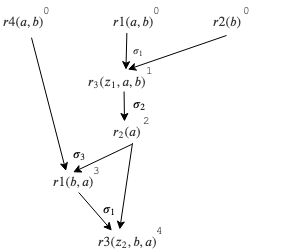
\includegraphics[scale=0.5]{chase_graph}
    \centering
\end{figure}

\end{exmp}


%% ...
\chapter{Resultados Formales}
\chapter{Implementación}

%%%% BIBLIOGRAFIA
\backmatter
\begin{thebibliography}{9}
    \bibitem{beeri} 
    C. Beeri y M. Y. Vardi.
    \textit{The implication problem for data dependencies}. 
    En \textit{Proc. ICALP-1981}, pp. 73–85, 1981.
     
    \bibitem{cali} 
    A. Calı, G. Gottlob, y M. Kifer.
    Taming the infinite chase: Query answering under expressive relational constraints.
    En \textit{Proc. KR-2008, pp. 70–80, 2008}. 

    \bibitem{Chandra} 
    A. K. Chandra and P. M. Merlin. 
    Optimal implementation of conjunctive queries in relational data bases.
    En \textit{Proc. KR-2008, pp. 70–80, 2008}. 

    \bibitem{Deutsch} 
    A. Deutsch, A. Nash, and J. B. Remmel.
    The chase revisited.
    En \textit{Proc. PODS-2008, pp. 149–158, 2008}. 

    \bibitem{Fagin} 
    R. Fagin, P. G. Kolaitis, R. J. Miller, and L. Popa.
    Data exchange: Semantics and query answering.
    En \textit{Theor. Comput. Sci., 336(1):89–124, 2005.}. 

    \bibitem{Johnson} 
    D. S. Johnson and A. C. Klug.
    Testing containment of conjunctive queries under functional and inclusion dependencies.
    En \textit{J. Comput. Syst. Sci., 28(1):167–189, 1984.}. 

    \end{thebibliography}

\end{document}
